\documentclass[12pt, a4paper, oneside]{ctexart}
\usepackage{amsmath, amsthm, amssymb, appendix, bm, graphicx, hyperref, mathrsfs}
\usepackage{verbatim}
\usepackage{multirow} % 引入multirow包
\usepackage{graphicx} %插入图片的宏包
\usepackage{float} %设置图片浮动位置的宏包
\usepackage{subfig} %插入多图时用子图显示的宏包

\graphicspath{ {./Figures/} }



\title{\textbf{给宝宝的考研择校}}
\author{PHDoet}
\date{\today}
\linespread{1.5}
\newtheorem{theorem}{定理}[section]
\newtheorem{definition}[theorem]{定义}
\newtheorem{lemma}[theorem]{引理}
\newtheorem{corollary}[theorem]{推论}
\newtheorem{example}[theorem]{例}
\newtheorem{proposition}[theorem]{命题}
\renewcommand{\abstractname}{\Large\textbf{摘要}}

\begin{document}

\maketitle

\setcounter{page}{0}
\thispagestyle{empty}

\begin{abstract}
    计算机专业考研人数众多,专业课内容多且难度大,选择一个合适的学校至关重要,
    这里我将列出一些与计算机交叉的学科以及一些相对比较好考的学校以供参考。
    \par\textbf{关键词:}研究生. 
\end{abstract}

\newpage
\pagenumbering{Roman}
\setcounter{page}{1}

\tableofcontents

\newpage
\setcounter{page}{1}
\pagenumbering{arabic}

\section{武汉大学}

    \subsection{网络法学(国家网络安全学院)}

以下是这个专业2024年的招生简章内容:
        \begin{table*}[h]
            \centering
            \caption{武汉大学网络法学}
            \begin{tabular}{|l|l|l|l|}
            \hline
                0301J1 网络法学 & 招生人数 & 初试科目 & 复试科目 \\
            \hline
                01 网络空间国际法 & \multirow{4}{*}{5} & 101 思想政治理论 & \multirow{4}{*}{网络法学} \\
            \cline{1-1}
                02 网络犯罪的法律治理 && 201 英语(一) & \\
            \cline{1-1}
                03 大数据与人工智能法律 && 657 网络技术基础 & \\
            \cline{1-1}
                04 数字经济的法律治理 && 824 法学基础B & \\
            \hline
            \end{tabular}
            \label{table_MAP}
        \end{table*}
    
        第一年专业课考察957网络技术基础+616法学综合(含法理、宪法、行政法、民法、刑法、国际法)。
        其中616系单独出题,刑法部分明显偏向网络法学与刑法的交叉部分。


        第二年专业课考察657网络技术基础+824法学基础B,下面介绍一下初试各科目情况:
\begin{enumerate}
    \item 101 思想政治理论
    \item 201 英语一
    \item 657 网络技术基础:主要考察内容是计算机网络,也包含部分计算机408的内容,参考书主要是谢希仁老师的《计算机网络》。
          对比该科目两年真题会发现,该科目的考察重点发生明显转向:
          \begin{enumerate}
            \item 第一年仅背诵即可拿分的名词解释、简答题占分高达80分,将基础知识点背会就可以拿到一个不错的分数;
                  第二年该类仅背诵即可拿分的题目占比明显减少,更加考察考生对于知识点的理解与掌握。
                  这提醒我们不可再用文科的思路去将知识点“背下来“,而是要用理科的思路将元知识点吃透,学会灵活运用.
            \item 第一年没有明显超纲的题目,考察的均为重点、较为基础的题目;
                  第二年超纲题高达二、三十分,且存在较难题目,出现了新题型。
                  例如计算题第一题的Di jkstra算法,在谢老师的书上是没有的,就算在计算机相关专业中也属于较难的知识点,
                  这提醒我们不可再局限于谢老师的书,而是要学会适当扩展。
          \end{enumerate}
    \item 824 法学基础B(含刑法学、民法学、国际公法学):22年与武汉大学法学院是同一张卷子,不再单独出题,
          这提醒我们不可按照第一年单独命题的思路仅关注与网络法交叉的内容,而是要按照法学院的命题思路全面复习
\end{enumerate}



\newpage
\section{中南财经政法大学}

\subsection{数字法学(国家治理学院)}

以下是2024年中南财经政法大学数字法学的招生简章,注意2024是其第一年招生。
\begin{table*}[h]
    \centering
    \caption{中南财经政法大学数字法学}
    \begin{tabular}{|l|l|l|l|}
    \hline
        专业名称 & 招生人数 & 初试科目 & 复试科目 \\
    \hline
        \multirow{4}{*}{数字法学} & \multirow{4}{*}{4} & 101 思想政治理论 & \multirow{4}{*}{1148 数字法学} \\
    
         && 201 英语(一) & \\
    
         && 616 法学基础 & \\
    
         && 856 数字法学 & \\
    \hline
    \end{tabular}
    \label{table_MAP}
\end{table*}


以下是数字法学专业课命题说明:
\begin{figure}[H] %H为当前位置,!htb为忽略美学标准,htbp为浮动图形
    \centering %图片居中
    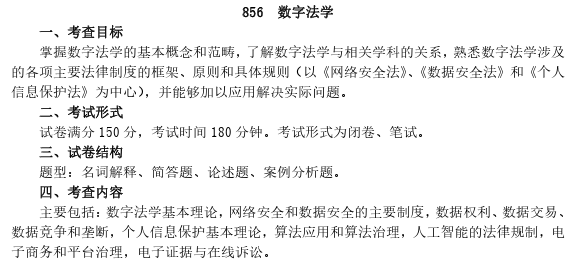
\includegraphics[width=\textwidth]{law} %插入图片,[]中设置图片大小,{}中是图片文件名
    \caption{数字法学} %最终文档中希望显示的图片标题
    \label{1}
\end{figure}





\begin{comment}
\newpage
\begin{thebibliography}{99}
    \bibitem{a}作者. \emph{文献}[M]. 地点:出版社,年份.
    \bibitem{b}作者. \emph{文献}[M]. 地点:出版社,年份.
\end{thebibliography}

\newpage

\begin{appendices}
    \renewcommand{\thesection}{\Alph{section}}
    \section{附录标题}
        这里是附录. 
\end{appendices}
\end{comment}

\end{document}